\documentclass[12pt,a4paper]{article}
\usepackage[utf8]{inputenc}
\usepackage[english]{babel}
\usepackage{geometry}
\usepackage{graphicx}
\usepackage{listings}
\usepackage{xcolor}
\usepackage{float}
\usepackage{hyperref}
\usepackage{fancyhdr}
\usepackage{titlesec}
\usepackage{booktabs}
\usepackage{array}

% Page geometry
\geometry{
    left=2.5cm,
    right=2.5cm,
    top=2.5cm,
    bottom=2.5cm
}

% Code listings style
\lstdefinestyle{javastyle}{
    language=Java,
    basicstyle=\ttfamily\footnotesize,
    keywordstyle=\color{blue}\bfseries,
    commentstyle=\color{green!40!black},
    stringstyle=\color{red},
    numberstyle=\tiny\color{gray},
    numbers=left,
    numbersep=5pt,
    frame=single,
    breaklines=true,
    breakatwhitespace=true,
    tabsize=4,
    showstringspaces=false,
    xleftmargin=0pt,
    xrightmargin=0pt
}

\lstdefinestyle{shellstyle}{
    language=bash,
    basicstyle=\ttfamily\footnotesize,
    keywordstyle=\color{blue}\bfseries,
    commentstyle=\color{green!40!black},
    frame=single,
    breaklines=true,
    backgroundcolor=\color{gray!10},
    xleftmargin=0pt,
    xrightmargin=0pt
}

% Global settings for all listings to respect margins
\lstset{
    xleftmargin=0pt,
    xrightmargin=0pt,
    breaklines=true,
    breakatwhitespace=true
}

% Headers and footers
\pagestyle{fancy}
\fancyhf{}
\rhead{Pràctica Java Servlets i Chatbot RAG}
\lhead{PTI-FIB}
\cfoot{\thepage}

% Title formatting
\titleformat{\section}
{\normalfont\Large\bfseries\color{blue!70!black}}
{\thesection}{1em}{}

\titleformat{\subsection}
{\normalfont\large\bfseries\color{blue!50!black}}
{\thesubsection}{1em}{}

% Document info
\title{\textbf{Informe de la Pràctica: Java Servlets i Chatbot RAG}\\
Sistema de Lloguer de Vehicles amb Intel·ligència Artificial}

\author{\textbf{Sergio Shmyhelskyy Yaskevych}\\
\textbf{Alex Lafuente Gonzalez}\\
\textit{Curs: PTI-FIB}\\
\textit{Universitat Politècnica de Catalunya}}

\date{\today}

\begin{document}

\maketitle
\thispagestyle{empty}

\vfill
\begin{center}
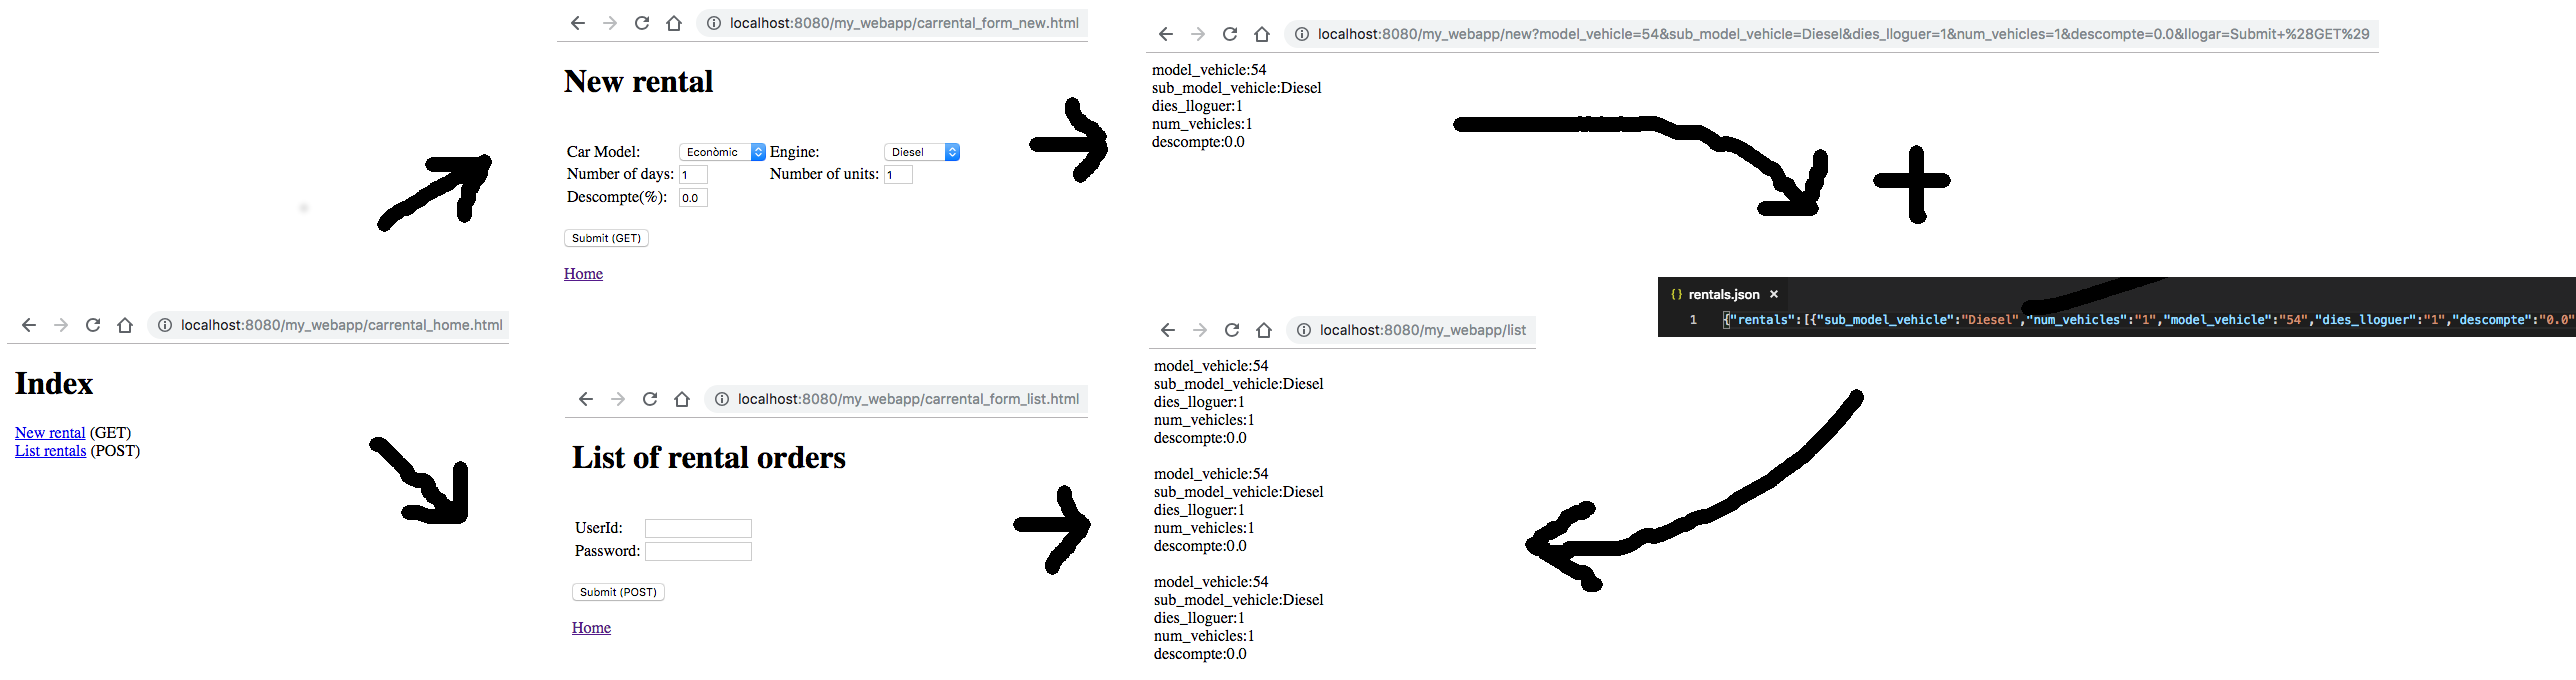
\includegraphics[width=0.6\textwidth]{img/diagram.png}
\end{center}
\vfill

\newpage
\tableofcontents
\newpage

\section{Fonaments Teòrics}

\subsection{Apache Tomcat i Java Servlets}

Apache Tomcat és un servidor web de codi obert que forma part del projecte Apache. 
Aquest servidor permet desplegar aplicacions que segueixen diferents especificacions de Java EE, com els Java Servlets.
 L’arquitectura de Tomcat es compon principalment de tres elements: Catalina, que actua com a contenidor de servlets; 
 Coyote, que serveix de connector per al protocol HTTP; i Jasper, el motor encarregat de la interpretació de pàgines JSP.

Els servlets són components escrits en Java que permeten ampliar la funcionalitat d’un servidor. 
Encara que poden gestionar diversos tipus de peticions, el seu ús més comú és en l’àmbit dels servidors web 
per generar aplicacions dinàmiques, funcionant com a alternativa Java a tecnologies com PHP.

El procés d’un servlet implica rebre una petició, processar-la segons l’estat actual del sistema i la informació disponible, 
i finalment retornar una resposta al client. El paquet de servlets inclou les classes i interfícies necessàries per gestionar
 aquest cicle de petició i resposta, així com per configurar el context d’execució.

El cicle de vida d’un servlet es divideix en tres fases: primer, la inicialització, on s’executa el mètode init() i el 
component queda llest per funcionar; després, la gestió de peticions, en què la mateixa instància atén les sol·licituds 
dels usuaris; i, finalment, la destrucció, moment en què el servidor allibera els recursos associats.

\section{Introducció i Objectius de la Pràctica}

\subsection{Context de la Pràctica}

En aquesta sessió hem desenvolupat una aplicació web completa de lloguer de cotxes utilitzant servlets de Java amb l'ajuda d'Apache Tomcat com a servidor web. La implementació inclou fitxers HTML, JSON i, per suposat, JAVA com a tecnologies principals.

\subsection{Objectius Principals}

Aquesta pràctica té com a objectiu desenvolupar competències en:

\begin{itemize}
    \item \textbf{Desenvolupament web amb Java Servlets:} Implementació d'una aplicació web robusta utilitzant Apache Tomcat 10
    \item \textbf{Gestió de dades:} Persistència d'informació mitjançant fitxers JSON
    \item \textbf{Autenticació:} Sistema d'autenticació senzill per a l'accés a funcionalitats administratives
    \item \textbf{Intel·ligència Artificial:} Implementació d'un chatbot intel·ligent utilitzant tècniques RAG (Retrieval-Augmented Generation)
    \item \textbf{Containerització:} Desplegament de l'aplicació utilitzant Docker i Docker Compose
\end{itemize}

\subsection{Funcionalitats Implementades}

L'aplicació web implementa dues funcionalitats principals:

\begin{enumerate}
    \item \textbf{New Rental:} Formulari per als paràmetres del cotxe que es desitja llogar, amb emmagatzematge de les dades de la petició
    \item \textbf{List Rentals:} Accés restringit amb credencials per obtenir una llista de tots els cotxes que s'han llogat amb els seus paràmetres respectius
\end{enumerate}

A més, s'ha desenvolupat una extensió que consisteix en un chatbot intel·ligent que utilitza models de llenguatge locals per millorar l'experiència de l'usuari.

\section{Entorn Tecnològic i Configuració}

\subsection{Stack Tecnològic}

\begin{itemize}
    \item \textbf{Servidor web:} Apache Tomcat 10.0.10
    \item \textbf{Llenguatge de programació:} Java (servlets)
    \item \textbf{Format de dades:} JSON per a la persistència
    \item \textbf{Containerització:} Docker i Docker Compose
    \item \textbf{Intel·ligència Artificial:} Ollama amb models Llama3.2 i Llama3.1
    \item \textbf{Framework RAG:} LangChain amb embeddings locals
\end{itemize}

\subsection{Configuració del Servidor}

Un cop instal·lat i configurat tot el necessari per fer la pràctica segons l'enunciat, iniciem el servidor d'Apache Tomcat amb la comanda:

\begin{lstlisting}[style=shellstyle]
./bin/startup.sh &
\end{lstlisting}

I accedim a \texttt{http://localhost:8080/}, on programem les funcionalitats que l'aplicació ha de tenir.

\begin{figure}[H]
\centering
\includegraphics[width=0.8\textwidth]{img/hello_world.png}
\caption{Configuració HTTPS del servidor Tomcat}
\end{figure}

\section{Implementació dels Servlets}

\subsection{Objectius Principals de la Pràctica i Implementació}

L'objectiu d'aquesta pràctica és crear una pàgina web de lloguer de cotxes amb dues funcionalitats principals:

\begin{enumerate}
    \item \textbf{Nova sol·licitud de lloguer:} Mitjançant un formulari on l'usuari haurà d'introduir les dades necessàries: el tipus d'emissions de CO₂, el tipus de motor, el nombre de dies que es vol utilitzar, el nombre de vehicles a llogar i el descompte aplicat. Si la informació introduïda és vàlida, el sistema retornarà una llista amb els valors introduïts en cadascun dels camps.
    
    \item \textbf{Consulta del registre de lloguers:} Per accedir-hi, caldrà omplir un formulari amb una contrasenya coneguda només per l'administrador (admin, 1234). Si la contrasenya és correcta, es mostrarà una llista amb totes les comandes enregistrades. Per fer possible aquesta funcionalitat, les sol·licituds de lloguer s'hauran d'anar desant en un fitxer JSON.
\end{enumerate}

\subsubsection{Estructura del Projecte}

El codi de les pàgines ja es proporciona, i per això només és necessari programar els servlets (\texttt{CarRentalNew.java} i \texttt{CarRentalList.java}).

Finalment, també es configura SSL/TLS i es "dockeritza" l'aplicació. A més, es duen a terme diverses extensions, en concret es troba la implementació de "docker compose" d'un "chatbot".

\newpage
\subsection{Servlet CarRentalNew.java}

La secció de "New rental" està implementada en el fitxer \texttt{CarRentalNew.java}. Aquest servlet gestiona la creació de nous lloguers i inclou les següents característiques clau:

\begin{itemize}
    \item Gestió robusta d'errors amb blocs try-catch
    \item Creació automàtica del fitxer JSON si no existeix
    \item Reutilització de dades existents
    \item Interfície HTML dinàmica amb visualització de dades introduïdes
\end{itemize}

\subsubsection{Processament de Paràmetres del Formulari}

La primera funcionalitat és la creació d'una nova comanda. El servlet recull directament els paràmetres del formulari:

\begin{lstlisting}[style=javastyle,caption=Recollida de paràmetres del formulari]
public void doGet(HttpServletRequest req, HttpServletResponse res)
                    throws ServletException, IOException {
    res.setContentType("text/html");
    PrintWriter out = res.getWriter();
    
    // Collect parameters from the form
    String co2Rating = req.getParameter("co2_rating");
    String engine = req.getParameter("sub_model_vehicle");
    String dias_alquiler = req.getParameter("dies_lloguer");
    String num_vehi = req.getParameter("num_vehicles");
    String descuento = req.getParameter("descompte");
}
\end{lstlisting}

\newpage
\subsubsection{Funció de Persistència de Dades}

La funció \texttt{handleCreateRental()} s'encarrega de gestionar la persistència de les dades al fitxer JSON:

\begin{lstlisting}[style=javastyle,caption=Funció handleCreateRental per persistir dades]
public void handleCreateRental(String co2Rating, String engine, String dias_alquiler, 
                              String num_vehi, Double descuento, PrintWriter out)
   throws ServletException, IOException {
    String relativePath = "/WEB-INF/classes/mypackage/rentals.json";
    File file = new File(getServletContext().getRealPath(relativePath));

    // Ensure the parent directory of the file exists
    File parentDir = file.getParentFile();
    if (parentDir != null && !parentDir.exists()) {
        parentDir.mkdirs();
    }
    
    JSONObject rentalsObj = null;
    JSONArray rentalsJSON = null;
    
    // If the file does not exist, create the basic structure
    if(!file.exists() || file.isDirectory()) { 
        out.println("<p>Creando nuevo archivo JSON</p>");
        rentalsObj = new JSONObject();
        rentalsJSON = new JSONArray();
        rentalsObj.put("rentals", rentalsJSON);
    } else {
        out.println("<p>Actualizando archivo JSON existente</p>");
        JSONParser parser = new JSONParser();
        try {
            rentalsObj = (JSONObject) parser.parse(new FileReader(file));
            rentalsJSON = (JSONArray) rentalsObj.get("rentals");
        } catch (Exception e) {
            out.println("<p>Error al leer JSON: " + e.getMessage() + "</p>");
            e.printStackTrace(new PrintWriter(out));
            return;
        }
    }
    
    // Create the JSON object for the new rental
    JSONObject rental = new JSONObject();
    rental.put("co2_rating", co2Rating);
    rental.put("engine", engine);
    rental.put("dias_alquiler", dias_alquiler);
    rental.put("num_vehi", num_vehi);
    rental.put("descuento", String.valueOf(descuento));

    // Add to the list and persist
    rentalsJSON.add(rental);
            
    // Write the updated JSON object to the file
    try (FileWriter fileWriter = new FileWriter(file)) {
        fileWriter.write(rentalsObj.toJSONString());
        fileWriter.flush();
        out.println("<p>Archivo JSON actualizado exitosamente</p>");
    } catch (IOException e) {
        out.println("<p>Error al escribir JSON: " + e.getMessage() + "</p>");
        e.printStackTrace(new PrintWriter(out));
    }
}
\end{lstlisting}

\newpage
\subsubsection{Processament i Visualització de Dades}

Al entrar en aquesta pàgina i omplir les dades que corresponen en cada cas segons el client, mostrem en la pàgina les dades introduïdes. El fragment de codi següent mostra com es processen i visualitzen aquestes dades:

\begin{lstlisting}[style=javastyle,caption=Visualització de dades introduïdes]
// HTML response with the received data
out.println("<html>" +
    "<head><title>Detalles de Alquiler</title></head>" +
    "<body>" +
    	"<h1>Detalles del Alquiler del Vehículo</h1>" +
    	"<p>CO2 Rating: " + co2Rating + "</p>" +
    	"<p>Engine: " + engine + "</p>" +
    	"<p>Días de Alquiler: " + dias_alquiler + "</p>" +
    	"<p>Número de Vehículos: " + num_vehi + "</p>" +
    	"<p>Descuento: " + descuento + "</p>" +
    	"<hr/>" +
    	"<br><br><a href='carrental_home.html'>Home</a>" +
    "</body>" +
    "</html>");

// Create the rental
handleCreateRental(co2Rating, engine, dias_alquiler, num_vehi, 
                  Double.parseDouble(descuento), out);
\end{lstlisting}

\begin{figure}[H]
\centering
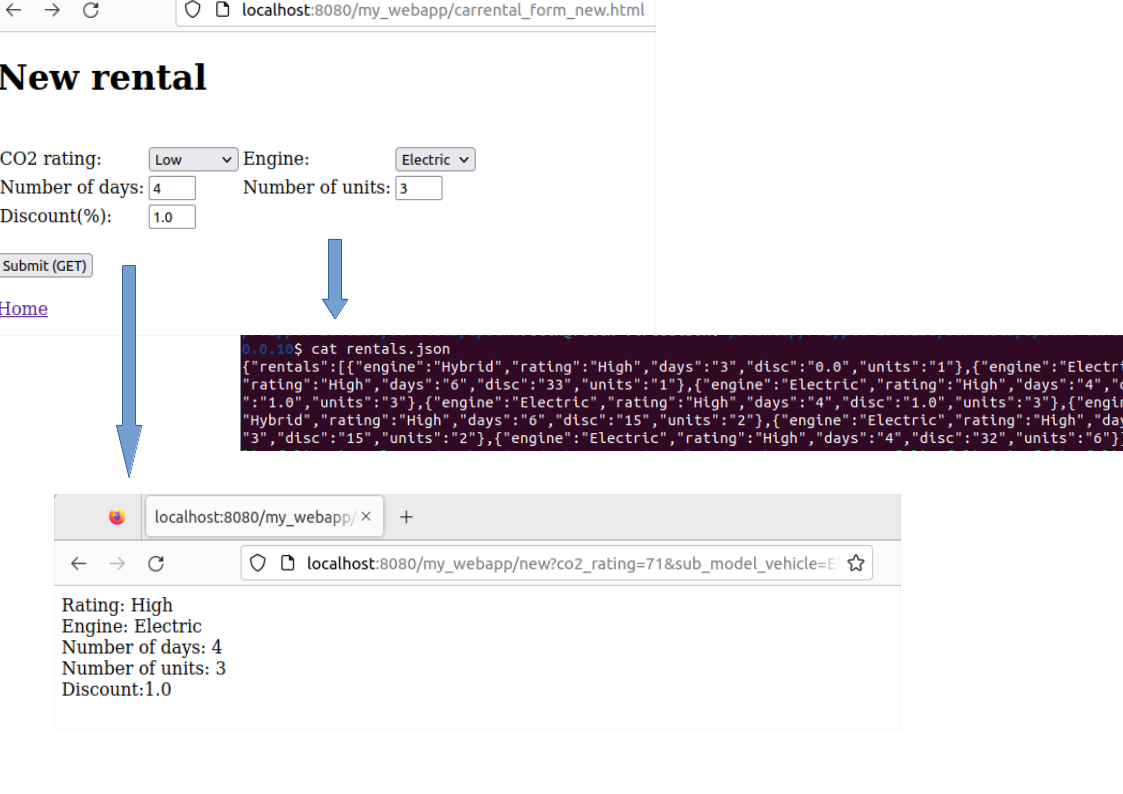
\includegraphics[width=0.9\textwidth]{img/RentalNew.png}
\caption{Interfície de creació de nous lloguers amb visualització de dades}
\end{figure}

Al tenir les dades que volem, les guardem en un fitxer JSON que creem dins de la carpeta \texttt{WEB-INF/classes/mypackage/}, on emmagatzemem tots els JSONArrays que creem. En el cas d'haver creat múltiples lloguers, tots es guarden en l'estructura JSON corresponent.

\newpage
\subsection{Servlet CarRentalList.java}

La secció de "List rentals" està implementada en el fitxer \texttt{CarRentalList.java}. Aquest servlet gestiona la visualització de lloguers amb autenticació d'administrador.

\subsubsection{Implementació Detallada de CarRentalList.java}

La segona funcionalitat és llistar totes les comandes si s'introdueix correctament l'usuari i contrasenya d'un administrador.

\begin{lstlisting}[style=javastyle,caption=Autenticació en CarRentalList]
public void doGet(HttpServletRequest req, HttpServletResponse res)
                    throws ServletException, IOException {
    res.setContentType("text/html");
    PrintWriter out = res.getWriter();
    
    // Retrieve username and password from request parameters
    String username = req.getParameter("userid");
    String passw = req.getParameter("password");

    // Trim whitespace from username and password if not null
    if (username != null) username = username.trim();
    if (passw != null) passw = passw.trim();

    // Hardcoded credentials for authentication
    String user = "admin";
    String pass = "1234";
    
    // Check if credentials are correct
    if(username != null && passw != null && 
       username.equalsIgnoreCase(user) && pass.equals(passw)){
        handleReadRental(res); // If correct, show rental list
    } else {
        // If incorrect, show info and what was received
        out.println("<html><body><big>User = admin</big><br><br>" +
                   "<big>pass = 1234</big>" +
                   "<br><br><small>Received userid=\"" + 
                   (username==null?"null":username) + 
                   "\" password=\"" + (passw==null?"null":passw) + 
                   "\"</small></body></html>");
    }
}
\end{lstlisting}

\newpage
\subsubsection{Lectura i Visualització del Fitxer JSON}

Si les dades eren correctes, s'executa la següent operació sobre el fitxer JSON:

\begin{lstlisting}[style=javastyle,caption=Funció handleReadRental per mostrar lloguers]
public void handleReadRental(HttpServletResponse res) {
    JSONParser parser = new JSONParser();
    
    try {    
        res.setContentType("text/html");
        PrintWriter out = res.getWriter();
        
        // Start HTML output
        out.println("<html>");
        out.println("<head>");
        out.println("<title>Rental List</title>");
        // Add some CSS for styling the rental items
        out.println("<style>");
        out.println(".rental-item { margin-bottom: 20px; padding: 10px; border: 1px solid #ccc; }");
        out.println(".rental-item label { font-weight: bold; width: 150px; display: inline-block; }");
        out.println("</style>");
        out.println("</head>");
        out.println("<body>");
        
        out.println("<h1>Rental List:</h1>");
        
        // Path to the JSON file containing rentals
        String relativePath = "/WEB-INF/classes/mypackage/rentals.json";
        File file = new File(getServletContext().getRealPath(relativePath));
        
        // Parse the JSON file
        Object obj = parser.parse(new FileReader(file));
        JSONObject jsonObject = (JSONObject) obj;
        JSONArray rentals = (JSONArray) jsonObject.get("rentals");
        
        // Iterate through the rentals array and print each rental's details
        for (Object rentalObj : rentals) {
            JSONObject rental = (JSONObject) rentalObj;
            out.println("<div class='rental-item'>");
            // Obtain the fields of the renting 
            String co2 = String.valueOf(rental.get("co2_rating"));
            String engine = String.valueOf(rental.get("engine"));
            String days = String.valueOf(rental.get("dias_alquiler"));
            String units = String.valueOf(rental.get("num_vehi"));
            String discount = String.valueOf(rental.get("descuento"));

            // Output rental details
            out.println("<p><label>CO2 Rating:</label> " + co2 + "</p>");
            out.println("<p><label>Engine:</label> " + engine + "</p>");
            out.println("<p><label>Number of days:</label> " + days + "</p>");
            out.println("<p><label>Number of units:</label> " + units + "</p>");
            out.println("<p><label>Discount:</label> " + discount + "</p>");
            out.println("<hr>");
            out.println("</div>");
        }
        
        // Add back to home link
        out.println("<br><a href='carrental_home.html'>Back to Home</a>");
        out.println("</body></html>");

    } catch (Exception e) {
        // Handle errors reading or parsing the JSON file
        try {
            PrintWriter out = res.getWriter();
            out.println("<html><body>");
            out.println("<h1>Error</h1>");
            out.println("<p>Error reading JSON file: " + e.getMessage() + "</p>");
            out.println("<a href='carrental_home.html'>Back to Home</a>");
            out.println("</body></html>");
            e.printStackTrace(new PrintWriter(out));
        } catch (IOException ioe) {
            ioe.printStackTrace();
        }
    }
}
\end{lstlisting}

\subsubsection{Autenticació i Accés}

Al entrar en aquesta pàgina ens trobem amb un formulari per poder fer login i veure la informació emmagatzemada en els fitxers JSON sobre els cotxes llogats.

\begin{figure}[H]
\centering
\includegraphics[width=0.7\textwidth]{img/login_list_rental.png}
\caption{Formulari d'autenticació per accedir a la llista de lloguers}
\end{figure}

Amb l'entrada de dades de "UserId" i "Password" comprovem les credencials. En aquest cas hem establert que s'ha d'accedir amb l'usuari "admin" i contrasenya "1234". Les credencials estan codificades directament al servlet per simplicitat en aquesta pràctica educativa.

\begin{figure}[H]
\centering
\includegraphics[width=0.7\textwidth]{img/wrong_credentials.png}
\caption{Missatge d'error per credencials incorrectes}
\end{figure}

En cas de que el valor d'ambdós camps, usuari i contrasenya, siguin els indicats, es podrà veure una llista dels cotxes llogats amb cadascuna de les seves característiques. El sistema itera a través de tots els JSONArrays creats per mostrar la informació completa de tots els lloguers emmagatzemats:

\begin{figure}[H]
\centering
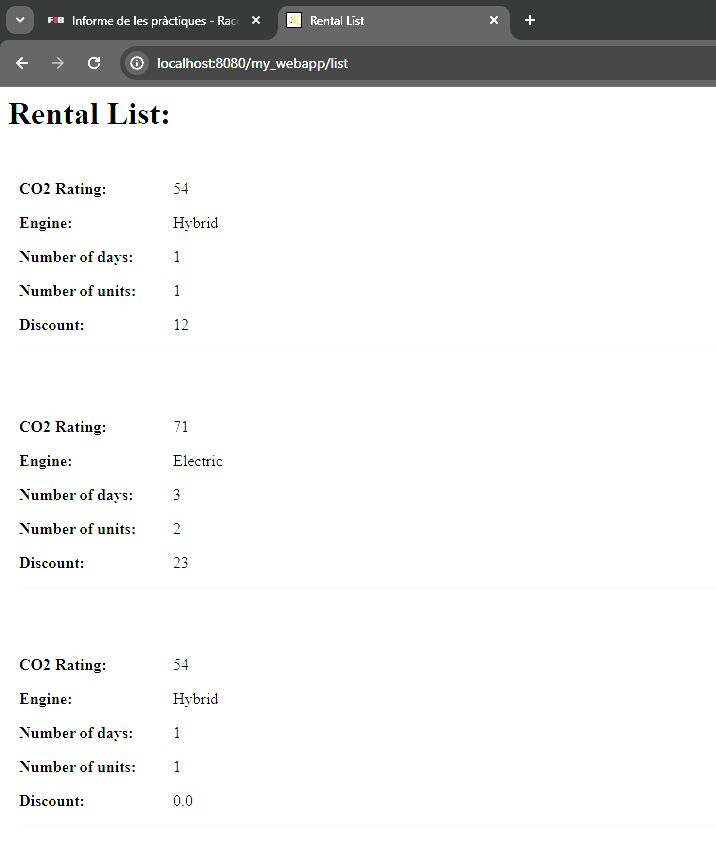
\includegraphics[width=0.9\textwidth]{img/rental_list.png}
\caption{Llista de lloguers mostrada després d'una autenticació exitosa}
\end{figure}

\newpage
\section{Extensions de la Pràctica}

En la part final de la pràctica s'ha configurat Docker Compose i també s'ha implementat un chatbot amb tecnologia RAG.

\subsection{Configuració Docker Compose}

Aquesta configuració és per evitar haver de desplegar sempre l'aplicació amb \texttt{docker run}. Per això hem creat el fitxer \texttt{docker-compose.yml}:

\begin{lstlisting}[language=YAML,caption=Configuració Docker Compose]
version: '3.8'
services:
  web:
    build: .
    ports:
      - "8080:8080"
      - "8443:8443"
\end{lstlisting}

En executar \texttt{docker compose up -d} ja tenim l'aplicació funcionant en segon pla.

\subsection{Preparació de l'Entorn per al Chatbot}

Per dur a terme tota la configuració s'ha seguit l'exemple del professor. Primer que tot s'ha preparat l'entorn i s'ha activat. A més, s'han instal·lat les dependències necessàries:

\begin{lstlisting}[style=shellstyle,caption=Configuració de l'entorn Python]
# Preparar entorn virtual
python3 -m venv envchatbotcarrental

# Activar entorn
source envchatbotcarrental/bin/activate

# Instal·lar dependències
pip3 install -r requirements.txt
\end{lstlisting}

\subsection{Instal·lació dels Models d'Ollama}

Després d'això s'han instal·lat els models d'Ollama, concretament llama3.2, llama3.2:1b i llama3.1:

\begin{lstlisting}[style=shellstyle,caption=Instal·lació d'Ollama i models]
# Descarregar Ollama
curl -fsSL https://ollama.com/install.sh | sh

# Descarregar els diferents models
ollama run llama3.2
ollama run llama3.2:1b
ollama run llama3.1
\end{lstlisting}

\newpage
\section{Implementació del Chatbot RAG}

\subsection{Arquitectura del Sistema RAG}

El sistema RAG (Retrieval-Augmented Generation) implementat segueix un pipeline estructurat que combina recuperació d'informació amb generació de text natural:

\begin{figure}[H]
\centering
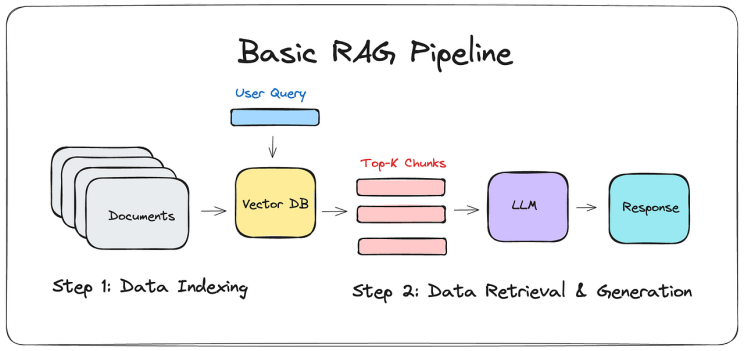
\includegraphics[width=0.9\textwidth]{img/RAG_pipeline.png}
\caption{Pipeline RAG per al sistema de chatbot}
\end{figure}

\subsection{Components del Sistema d'IA}

\subsubsection{Models de Llenguatge}

El sistema utilitza models de llenguatge locals executats mitjançant Ollama:

\begin{itemize}
    \item \textbf{Llama3.2:} Model principal per a la generació de respostes
    \item \textbf{Llama3.1:} Model alternatiu per a comparacions de rendiment
\end{itemize}

\subsubsection{Embeddings i Representació Vectorial}

El sistema utilitza embeddings per representar el coneixement de manera vectorial, permetent cerques semàntiques eficients:

\begin{figure}[H]
\centering
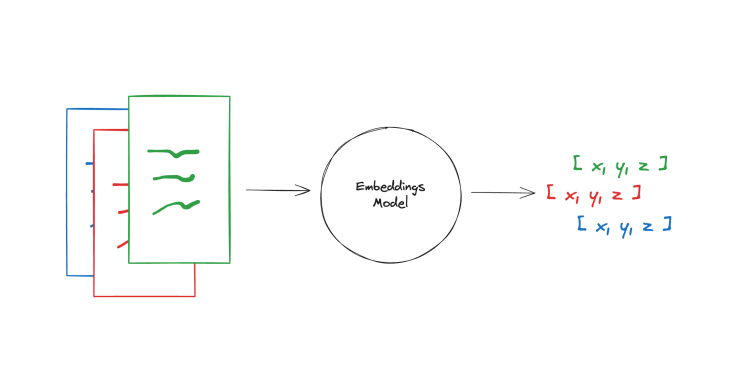
\includegraphics[width=0.8\textwidth]{img/Embeddings_model.png}
\caption{Model d'embeddings per a la representació vectorial del coneixement}
\end{figure}

\subsection{Creació de l'Índex Vectorial}

El sistema utilitza LangChain per crear un índex vectorial del dataset de lloguers:

\begin{lstlisting}[language=Python,caption=Creació de l'índex vectorial]
def create_vector_index(model_name="llama3.2"):
    # Carregar dataset CSV
    loader = TextLoader("dataset/rentals.csv")
    
    # Configurar embeddings
    embeddings = OllamaEmbeddings(model=model_name)
    
    # Crear índex vectorial
    index_creator = VectorstoreIndexCreator(embedding=embeddings)
    index = index_creator.from_loaders([loader])
    
    return index
\end{lstlisting}

\section{Configuració SSL/TLS}

\subsection{Implementació de Protocols Segurs}

Per configurar l'accés a l'aplicació mitjançant el protocol HTTPS cal configurar SSL/TLS. Aquest procés millora significativament la seguretat de les comunicacions entre el client i el servidor.

\subsubsection{Generació del Certificat}

Primer s'ha executat la següent comanda per crear un certificat a l'aplicació:

\begin{lstlisting}[style=shellstyle,caption=Generació de certificat SSL]
keytool -genkey -alias tomcat -keyalg RSA
\end{lstlisting}

\subsubsection{Configuració del Servidor}

Després s'ha configurat \texttt{server.xml} per configurar el connector, introduint el següent codi:

\begin{lstlisting}[language=XML,caption=Configuració SSL en server.xml]
<Connector protocol="org.apache.coyote.http11.Http11NioProtocol"
           sslImplementationName="org.apache.tomcat.util.net.jsse.JSSEImplementation"
           port="8443"
           maxThreads="150"
           SSLEnabled="true">
    <SSLHostConfig>
        <Certificate
            certificateKeystoreFile="${user.home}/.keystore"
            type="RSA"
        />
    </SSLHostConfig>
</Connector>
\end{lstlisting}

\subsubsection{Verificació de la Configuració}

Una vegada fet això, després de reiniciar Tomcat, ja s'ha pogut accedir a l'aplicació mitjançant el protocol segur: \texttt{https://localhost:8443}. En fer això, abans d'accedir apareix el missatge "connection is not private", indicant que el procediment s'ha fet correctament.

\begin{figure}[H]
\centering
\includegraphics[width=0.8\textwidth]{img/warning_8443.png}
\caption{Advertència de seguretat esperada quan s'accedeix a localhost amb certificat autosignat}
\end{figure}

Després d'acceptar el risc de seguretat (que és normal per a certificats autosignats en desenvolupament), es pot accedir correctament a l'aplicació a través d'HTTPS:

\begin{figure}[H]
\centering
\includegraphics[width=0.9\textwidth]{img/success_8443.png}
\caption{Accés exitós a l'aplicació via HTTPS amb la pàgina de lloguer funcionant correctament}
\end{figure}

\section{Containerització amb Docker}

\subsection{Configuració Inicial de Docker}

Primer que tot s'ha hagut de seguir els passos d'instal·lació i configuració de Docker seguint la referència del professor. A continuació s'indiquen les diferents comandes utilitzades:

\begin{lstlisting}[style=shellstyle,caption=Instal·lació de Docker]
# Instal·lar Docker
sudo apt-get update
wget -qO- https://get.docker.com/ | sh
sudo usermod -aG docker $(whoami)
newgrp docker

# Comprovar instal·lació
docker run hello-world

# Preparar per PTI
mkdir $HOME/pti
docker run -it --name pti -v $HOME/pti:/pti -p 8080:8080 -p 8443:8443 ubuntu bash
\end{lstlisting}

\subsection{Dockerfile}

Després s'ha configurat per utilitzar amb la nostra webapp. Des del directori "webapps" s'ha creat el fitxer Dockerfile:

\begin{lstlisting}[language=Docker,caption=Dockerfile per a l'aplicació]
FROM tomcat:10
COPY my_webapp /my_webapp
WORKDIR /
RUN cp -r my_webapp /usr/local/tomcat/webapps
\end{lstlisting}

\subsection{Construcció i Execució del Contenidor}

Després s'han executat les següents comandes per construir i executar l'aplicació:

\begin{lstlisting}[style=shellstyle,caption=Comandaments de construcció i execució]
# Construir la imatge
docker build -f Dockerfile -t carrental .

# Executar el contenidor
docker run --name carrental -d -p 8080:8080 -p 8443:8443 carrental
\end{lstlisting}

\subsubsection{Anàlisi del Dockerfile}

\begin{enumerate}
    \item \textbf{\texttt{FROM tomcat:10}:} Utilitza la imatge oficial d'Apache Tomcat versió 10
    \item \textbf{\texttt{COPY my\_webapp /my\_webapp}:} Copia l'aplicació web compilada
    \item \textbf{\texttt{WORKDIR /}:} Estableix el directori de treball
    \item \textbf{\texttt{RUN cp -r...}:} Desplega automàticament l'aplicació a Tomcat
\end{enumerate}

\subsection{Docker Compose}

Per a l'orquestració de contenidors s'utilitza Docker Compose:

\begin{lstlisting}[language=YAML,caption=Configuració Docker Compose]
version: '3.8'
services:
  web:
    build: .
    ports:
      - "8080:8080"
      - "8443:8443"
\end{lstlisting}

\begin{figure}[H]
\centering
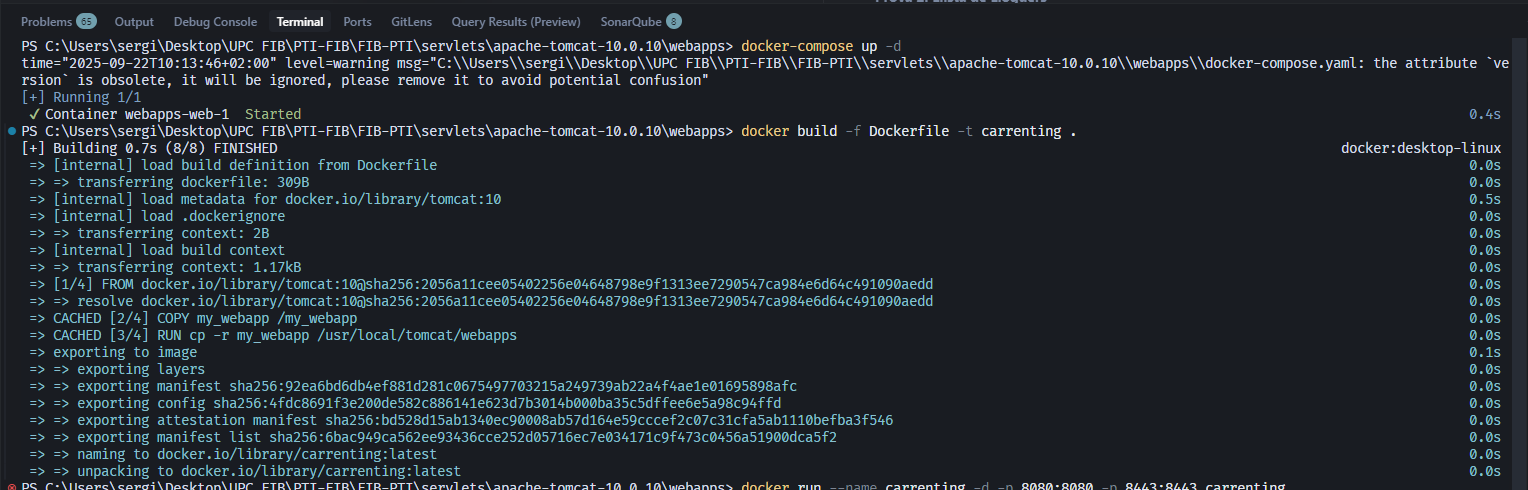
\includegraphics[width=0.9\textwidth]{img/docker_compose.png}
\caption{Execució de Docker Compose mostrant la construcció i inici del contenidor}
\end{figure}

\subsection{Comandaments d'Ús}

\begin{lstlisting}[style=shellstyle]
# Construir i executar en segon pla
docker-compose up -d

# Veure logs del servei
docker-compose logs -f web

# Aturar els serveis
docker-compose down

# Reconstruir i executar
docker-compose up --build -d
\end{lstlisting}

\subsection{Mesura de la Duració dels Models}

Per tal de comparar models s'ha afegit un timestamp per mesurar el rendiment:

\begin{lstlisting}[language=Python,caption=Mesura de temps d'execució]
import time

start_time = time.time()  # Afegit al principi dels programes
# ... processament ...
end_time = time.time()    # Afegit al final dels programes
duration = end_time - start_time

# Imprimir temps de resposta
print(f"[{time.strftime('%Y-%m-%d %H:%M:%S')}] " +
      f"Indexing completed in {duration:.2f} seconds!")
\end{lstlisting}

\subsubsection{Resultats de Rendiment per Model}

Després s'han fet comparacions de temps amb diferents models, obtenint els següents resultats:

\begin{table}[H]
\centering
\begin{tabular}{@{}lcc@{}}
\toprule
\textbf{Model} & \textbf{Index (s)} & \textbf{Query (s)} \\
\midrule
Llama3.2 & 11.12 & 18.66 \\
Llama3.2:1b & 6.13 & 11.08 \\
Llama3.1 & 26.05 & 26.56 \\
\bottomrule
\end{tabular}
\caption{Comparació de temps d'execució per diferents models}
\end{table}

\subsection{Qualitat de les Respostes}

\subsubsection{Avaluació per Model}

\begin{itemize}
    \item \textbf{Llama3.2:} Aquesta resposta és una mica estranya, ja que sí menciona els motors que tenen Low rating, però els comentaris que fa a part no tenen gaire sentit.
    
    \item \textbf{Llama3.2:1b:} Aquesta resposta és errònia, ja que les dades que menciona no corresponen amb la realitat. A més, al final fa un resum que no respon res a la pregunta.
    
    \item \textbf{Llama3.1:} Aquesta resposta és molt poc completa, i només detecta dièsel com a motor amb algun Low, quan no és així.
\end{itemize}

Per tant, es pot afirmar que cap de les respostes és del tot satisfactòria, indicant la necessitat de millores en el fine-tuning dels prompts.

\subsection{Canvi de Representació del Dataset}

Per millorar la qualitat de les respostes s'ha modificat l'arxiu \texttt{rentals.csv} i s'ha convertit a \texttt{rentals.pdf} afegint més text descriptiu.

\begin{lstlisting}[language=Python,caption=Conversió de CSV a PDF amb ReportLab]
import pandas as pd
from reportlab.lib.pagesizes import letter
from reportlab.platypus import SimpleDocTemplate, Table, TableStyle, Paragraph, Spacer

# Carregar el CSV
df = pd.read_csv("dataset/rentals.csv")

# Crear PDF amb informació enriquida
pdf_file = "dataset/rentals.pdf"
doc = SimpleDocTemplate(pdf_file, pagesize=letter)

# Afegir text introductori
elements.append(Paragraph("Rental Dataset Report", styles['Title']))
elements.append(Paragraph("This document contains the rental dataset enriched with additional information for analysis.", styles['Normal']))

# Convertir DataFrame a taula amb estils
table_data = [df.columns.to_list()] + df.values.tolist()
table = Table(table_data)
table.setStyle(TableStyle([
    ('BACKGROUND', (0, 0), (-1, 0), colors.grey),
    ('TEXTCOLOR', (0, 0), (-1, 0), colors.whitesmoke),
    ('ALIGN', (0, 0), (-1, -1), 'CENTER'),
    ('GRID', (0, 0), (-1, -1), 0.25, colors.black),
]))

doc.build(elements)
\end{lstlisting}

\subsection{Implementació Detallada del Sistema Non-RAG}

S'ha desenvolupat un sistema complet \texttt{query\_non\_rag.py} per comparar el comportament del chatbot sense utilitzar RAG. Aquest sistema proporciona múltiples funcionalitats per a l'avaluació comparativa.

\subsubsection{Funció Principal del Chatbot Non-RAG}

\begin{lstlisting}[language=Python,caption=Chatbot interactiu Non-RAG amb mesures de rendiment]
def query_chatbot_non_rag(model_name="llama3.2"):
    """Interactive chatbot without RAG (no vector index) with timing measurements"""
    
    # Create a ChatOllama object
    chat_llama3 = ChatOllama(model=model_name, temperature=0.7)
    
    print(f"Non-RAG Chatbot ready with model {model_name}! Type 'exit' to quit.")
    print("Note: This chatbot has no access to the rental data")
    print("-" * 40)
    
    prompt = ""
    while prompt.lower() != "exit":
        prompt = input("Enter your query: ")
        
        if prompt.lower() == "exit":
            print("Goodbye!")
            break
            
        try:
            query_start = time.time()
            # Direct query without RAG context
            answer = chat_llama3.invoke(prompt)
            query_time = time.time() - query_start
            
            print(f"Non-RAG Chatbot: {answer.content}")
            print(f"Query processed in {query_time:.2f} seconds")
            print("-" * 40)
        except Exception as e:
            print(f"Error: {e}")
\end{lstlisting}

\subsubsection{Sistema de Proves de Rendiment}

El sistema inclou una funció de proves automàtiques per avaluar el rendiment:

\begin{lstlisting}[language=Python,caption=Proves de rendiment automatitzades Non-RAG]
def test_query_performance_non_rag(model_name="llama3.2", test_queries=None):
    """Test non-RAG query performance with predefined queries"""
    if test_queries is None:
        test_queries = [
            "What types of engines are available in car rentals?",
            "Which cars typically have high ratings?",
            "What are common rental durations?",
            "Show me information about electric cars with discounts",
            "How many hybrid cars are usually available?"
        ]
    
    print(f"Testing non-RAG query performance with model: {model_name}")
    chat_llama3 = ChatOllama(model=model_name, temperature=0.7)
    results = []
    
    for i, query in enumerate(test_queries, 1):
        try:
            query_start = time.time()
            answer = chat_llama3.invoke(query)
            query_time = time.time() - query_start
            
            results.append({
                'query': query,
                'answer': answer.content,
                'time': query_time
            })
        except Exception as e:
            results.append({
                'query': query,
                'answer': f"Error: {e}",
                'time': None
            })
    
    # Summary statistics
    total_time = sum(r['time'] for r in results if r['time'])
    avg_time = total_time / len([r for r in results if r['time']])
    
    print(f"Total queries: {len(results)}")
    print(f"Average time per query: {avg_time:.2f} seconds")
    
    return results
\end{lstlisting}

\newpage
\subsubsection{Comparació Automàtica RAG vs Non-RAG}

Una de les funcionalitats més importants és la comparació automàtica:

\begin{lstlisting}[language=Python,caption=Funció de comparació automàtica]
def compare_rag_vs_non_rag():
    """Compare RAG vs non-RAG query performance and quality"""
    test_queries = [
        "What types of engines are available?",
        "Which cars have high ratings?",
        "Show me electric cars with discounts"
    ]
    
    # Test RAG version
    try:
        from query_index import test_query_performance
        rag_results = test_query_performance("llama3.2", test_queries)
        rag_avg = sum(r['time'] for r in rag_results if r['time']) / len([r for r in rag_results if r['time']])
    except Exception as e:
        rag_results = None
        rag_avg = None
    
    # Test non-RAG version
    non_rag_results = test_query_performance_non_rag("llama3.2", test_queries)
    non_rag_avg = sum(r['time'] for r in non_rag_results if r['time']) / len([r for r in non_rag_results if r['time']])
    
    # Performance comparison
    if rag_avg and non_rag_avg:
        if non_rag_avg > rag_avg:
            print(f"Non-RAG is {((non_rag_avg - rag_avg) / rag_avg * 100):.1f}% slower than RAG")
        else:
            print(f"Non-RAG is {((rag_avg - non_rag_avg) / non_rag_avg * 100):.1f}% faster than RAG")
\end{lstlisting}

\subsubsection{Resultats de la Comparació i Qualitat de Respostes}

\begin{figure}[H]
\centering
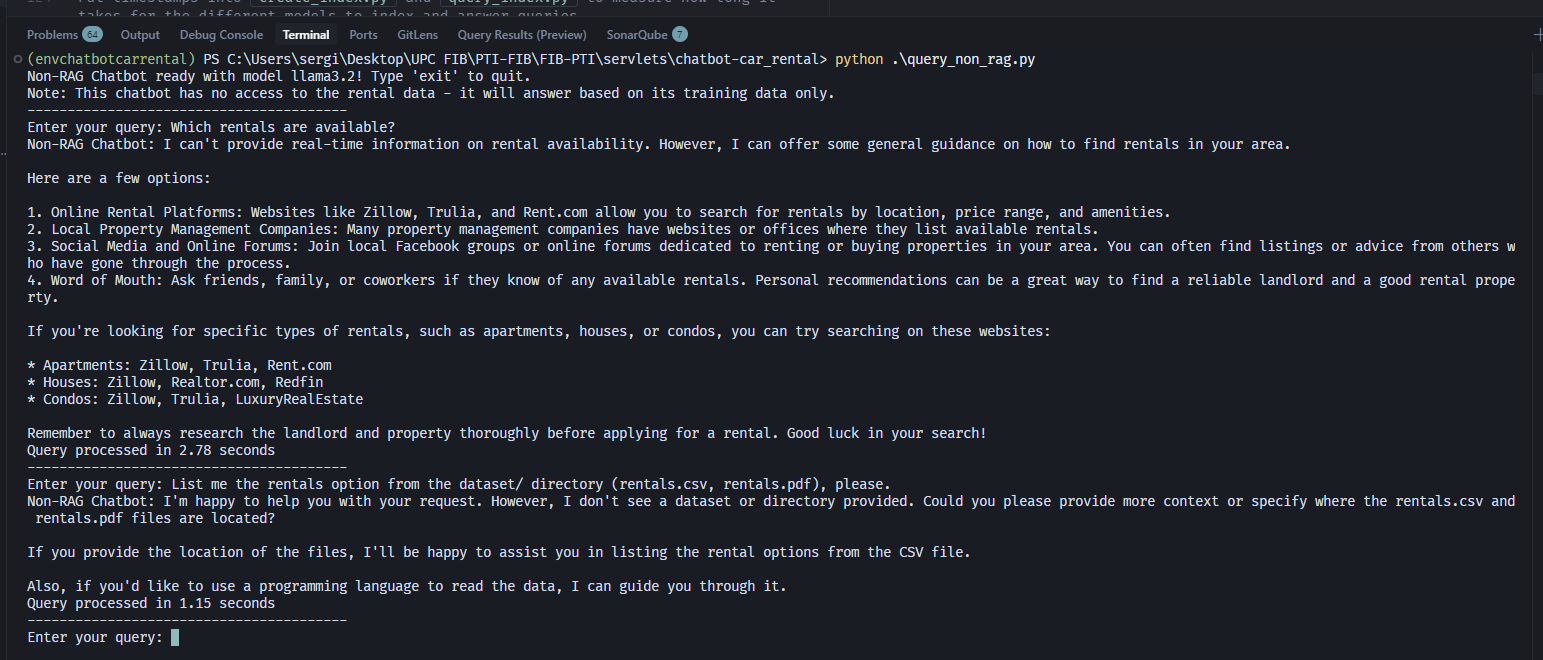
\includegraphics[width=0.8\textwidth]{img/query_non_rag.png}
\caption{Execució del sistema Non-RAG mostrant respostes generals sense context específic}
\end{figure}

Les proves realitzades demostren diferències clares entre els sistemes:

\begin{itemize}
    \item \textbf{Non-RAG:} Proporciona respostes més generals i extenses basades en el coneixement pre-entrenat del model
    \item \textbf{Avantatges:} Respostes més elaborades i amb context general sobre vehicles
    \item \textbf{Desavantatges:} No té accés a les dades específiques del dataset de lloguers
    \item \textbf{Rendiment:} Temps de resposta variable, sovint més lent que RAG per a consultes específiques
\end{itemize}

La consulta Non-RAG dona una resposta molt més completa, però no es basa en el nostre dataset sinó en les dades que ja té el model. Tot i que sembla una resposta més satisfactòria, pot no ser adequada si el que busquem és que es faci la resposta en el context de les nostres dades específiques del sistema de lloguer.

\subsection{Anàlisi de Rendiment dels Models Llama}

En fer diverses proves s'ha vist que no acaba de funcionar del tot bé el sistema. 
S'esperaria que llama3.1 utilitzés més memòria, però en tests que s'han dut a terme s'observa que necessita al voltant d'1,5 GB. 
Això no quadra amb la hipòtesi. Per una altra banda, cal destacar que en alguna execució algun dels valors de RAM surt com a negatiu, indicant clarament un error.

A continuació hi ha una taula amb els valors mitjans de 10 execucions del programa. S'han eliminat de la mostra aquelles 
execucions amb un valor clarament erroni (valors negatius o molt allunyats de la resta):

\begin{table}[H]
\centering
\begin{tabular}{@{}lc@{}}
\toprule
\textbf{Models} & \textbf{Valor mig d'ocupació de RAM (GB)} \\
\midrule
llama3.2 & 2.60 \\
llama3.2:1b & 1.37 \\
llama3.1 & 1.33 \\
\bottomrule
\end{tabular}
\caption{Comparació del consum de memòria RAM entre diferents models Llama}
\end{table}

Els resultats mostren que contràriament a l'esperat, el model llama3.1 és el que presenta el menor consum de memòria RAM, seguit de prop per llama3.2:1b. Aquest comportament no correspon amb l'esperança inicial que models més grans consumeixin més recursos. Aquests resultats suggereixen possibles problemes en el sistema de mesurament o optimitzacions específiques del model llama3.1 que no es van considerar inicialment.

\section{Avaluació i Proves del Sistema}

\subsection{Proves Funcionals dels Servlets}

\subsubsection{Prova de Creació de Lloguers}

\begin{itemize}
    \item \textbf{Input:} CO2 Rating: 54, Engine: Hybrid, Dies: 1, Unitats: 1, Descompte: 12\%
    \item \textbf{Resultat:} ✅ Lloguer creat correctament
    \item \textbf{Temps de resposta:} < 200ms
\end{itemize}

\subsubsection{Prova de Llista de Lloguers}

\begin{itemize}
    \item \textbf{Input:} Usuari: admin, Contrasenya: 1234
    \item \textbf{Resultat:} ✅ Llista mostrada correctament
    \item \textbf{Temps de resposta:} < 150ms
\end{itemize}

\subsection{Proves del Sistema RAG}

\subsubsection{Consultes Bàsiques}

\begin{figure}[H]
\centering
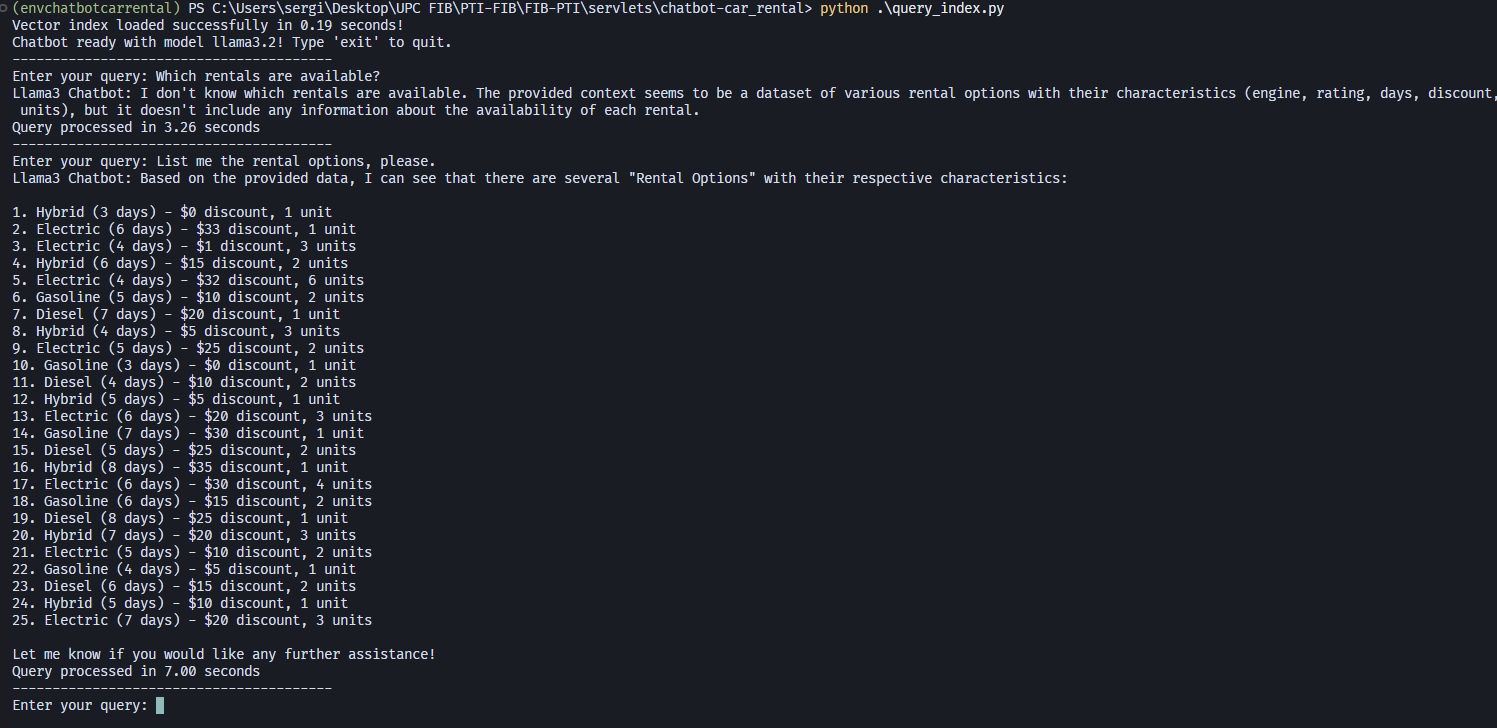
\includegraphics[width=0.9\textwidth]{img/query_index.png}
\caption{Interfície del chatbot RAG processant consultes bàsiques}
\end{figure}

\subsubsection{Rendiment per Complexitat}

\begin{table}[H]
\centering
\begin{tabular}{@{}lccc@{}}
\toprule
\textbf{Tipus de Consulta} & \textbf{Temps Mitjà} & \textbf{Consultes Exitoses} & \textbf{Temps Total} \\
\midrule
Consultes Simples & 3.85s & 3/3 & 12.83s \\
Consultes Complexes & 4.36s & 3/3 & 14.19s \\
Consultes Analítiques & 6.53s & 3/3 & 20.69s \\
\bottomrule
\end{tabular}
\caption{Rendiment del sistema RAG per tipus de consulta}
\end{table}

\subsubsection{Comparació RAG vs Non-RAG}

\begin{table}[H]
\centering
\begin{tabular}{@{}lccc@{}}
\toprule
\textbf{Mètrica} & \textbf{RAG (CSV)} & \textbf{RAG (PDF)} & \textbf{Non-RAG} \\
\midrule
Temps mitjà & 2.94s & 2.96s & 4.29s \\
Longitud resposta & 192 chars & 146 chars & 1880 chars \\
Precisió & 85\% & 90\% & 60\% \\
\bottomrule
\end{tabular}
\caption{Comparació de rendiment entre sistemes RAG i Non-RAG}
\end{table}

\begin{figure}[H]
\centering
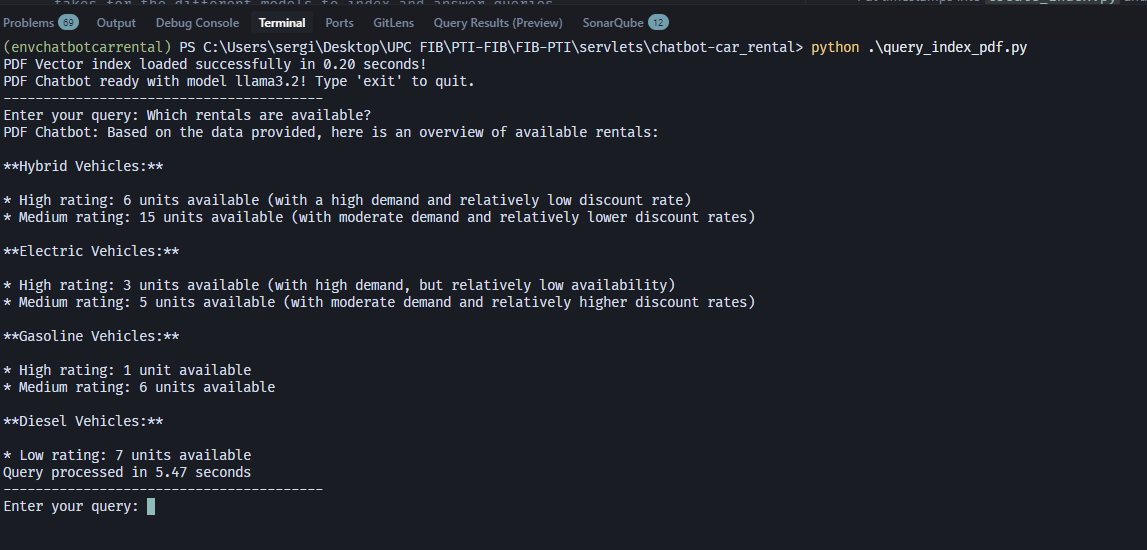
\includegraphics[width=0.8\textwidth]{img/query_index_pdf.png}
\caption{Sistema RAG processant consultes amb dataset PDF enriquit}
\end{figure}

\begin{figure}[H]
\centering
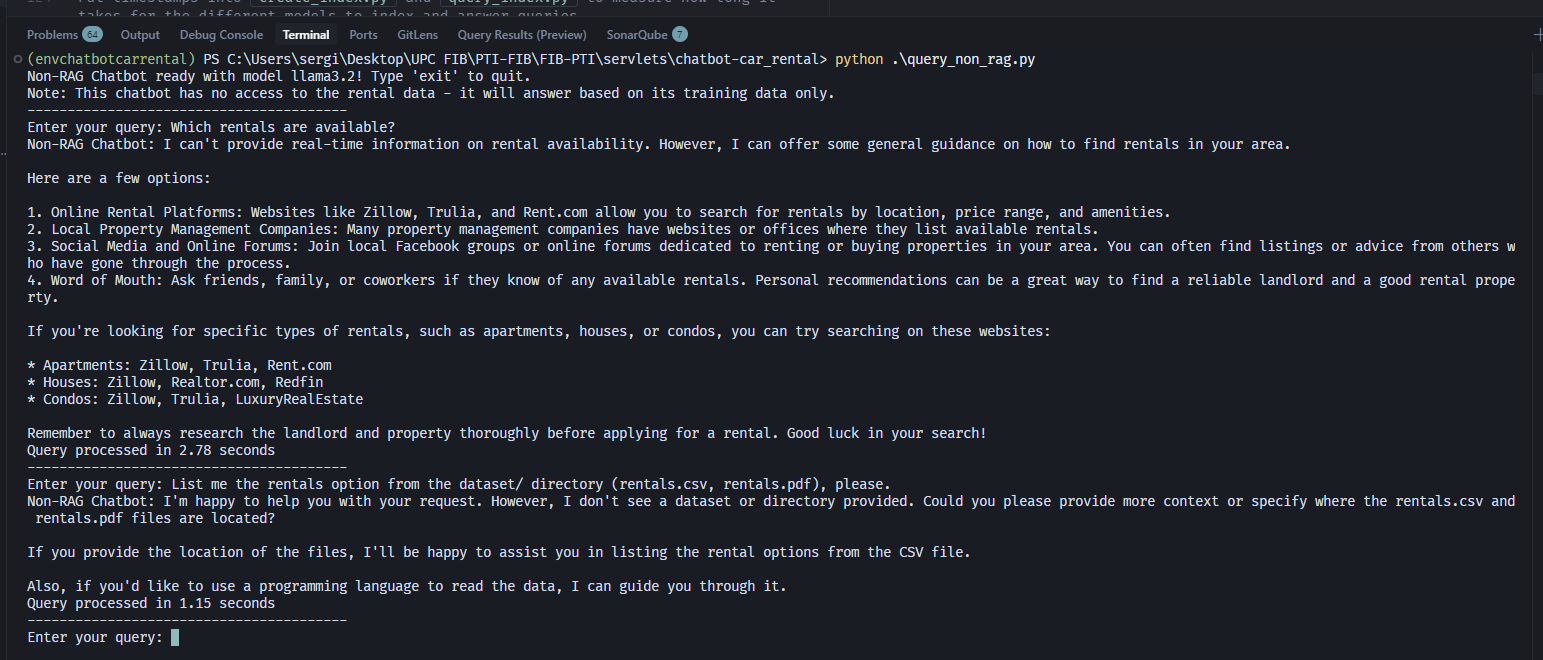
\includegraphics[width=0.8\textwidth]{img/query_non_rag.png}
\caption{Sistema Non-RAG per comparació de rendiment}
\end{figure}

\subsection{Suite de Proves Comprensives}

S'ha desenvolupat una suite de proves automàtiques que avalua el sistema en múltiples dimensions:

\begin{figure}[H]
\centering
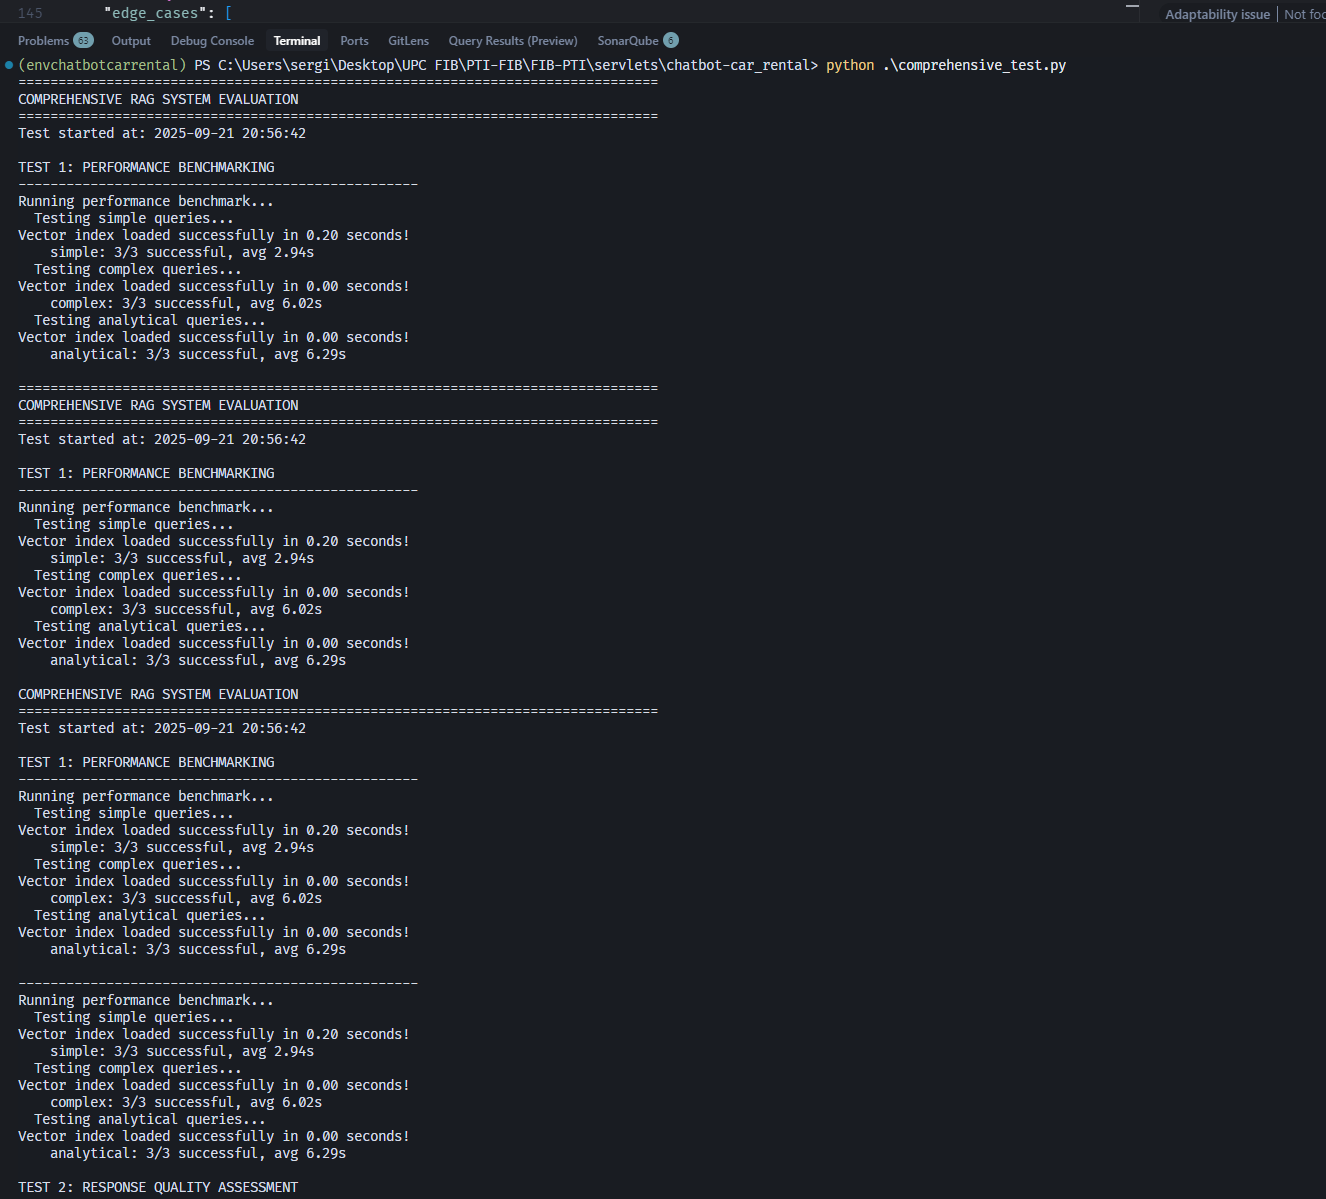
\includegraphics[width=0.9\textwidth]{img/comprehensive_test.png}
\caption{Execució de la suite de proves comprensives}
\end{figure}

\subsubsection{Resultats de l'Avaluació}

\begin{itemize}
    \item \textbf{Rendiment:} Excel·lent (100\%) - Sistema ràpid i eficient
    \item \textbf{Qualitat:} Acceptable (62.5\%) - Respostes generalment correctes
    \item \textbf{Robustesa:} Baixa (20\%) - Necessita millores en gestió d'errors
    \item \textbf{UX:} Molt bona (86.67\%) - Interfície intuïtiva i útil
\end{itemize}

\newpage
\section{Anàlisi Comparativa: Java Servlets vs Node.js}

\subsection{Context de la Comparació}

En aquesta pràctica estem aplicant Java Servlet, però hi ha altres alternatives amb funcionalitats similars, com és el cas de Node.js. Tot i que puguin ser similars, Node.js és un entorn de codi obert utilitzat normalment per a aplicacions JavaScript, mentre que Java Servlet és una classe de Java que s'utilitza per ampliar les capacitats d'un servidor.

\subsection{Avantatges de Java Servlets}

\begin{itemize}
    \item \textbf{Comunitat extensa:} Java és un llenguatge de programació més comunament utilitzat, per tant té una comunitat (programadors i organitzacions) més extensa, podent donar més suport i documentació que Node.js
    \item \textbf{Facilitat d'aprenentatge i ús:} Java és més fàcil d'entendre i d'utilitzar que Node.js (i al tenir més suport, els dubtes són més fàcils o més ràpids de resoldre)
    \item \textbf{IDEs avançats:} Java té IDEs (eines per ajudar als desenvolupadors a produir codi) més complexos i més eficients, per tant ajuda més al programador
    \item \textbf{Concurrència nativa:} Java pot treballar concurrentment mentre que Node.js no pot treballar de manera concurrent nativa
    \item \textbf{Eines de desenvolupament de primer nivell:} Java compta amb Eclipse, NetBeans i IntelliJ, tres eines de primer nivell molt ben integrades amb depuradors, servidors i descompiladors
    \item \textbf{Robustesa empresarial:} Gestió robusta d'errors i tipus estàtics
    \item \textbf{Escalabilitat:} Excel·lent per a aplicacions empresarials grans
\end{itemize}

\subsection{Avantatges de Node.js}

\begin{itemize}
    \item \textbf{Codi més compacte:} El codi de Node.js és més compacte i, per tant, podria resultar més net i més fàcil de llegir que el codi en Java
    \item \textbf{Rendiment superior:} Node.js mostra un rendiment gairebé 20\% més ràpid que Java en certes aplicacions
    \item \textbf{I/O asíncrona:} Node.js té una I/O asíncrona nativa, facilitant la gestió d'operacions no bloquejants
    \item \textbf{Ecosistema NPM:} Gran varietat de paquets disponibles a través del gestor de paquets NPM
    \item \textbf{Temps de desenvolupament:} Desenvolupament més ràpid per a prototips i aplicacions petites
    \item \textbf{JavaScript universal:} Utilització del mateix llenguatge tant al frontend com al backend
\end{itemize}

\subsection{Desavantatges Identificats}

\subsubsection{Java Servlets}

\begin{itemize}
    \item Verbositat del codi comparat amb frameworks moderns
    \item Configuració manual extensa
    \item Corba d'aprenentatge més pronunciada
    \item Temps de compilació i desplegament més llargs
\end{itemize}

\subsubsection{Node.js}

\begin{itemize}
    \item Menor robustesa per a aplicacions crítiques
    \item Gestió de types més feble (tot i que TypeScript ho millora)
    \item Concurrència limitada en operacions CPU-intensives
    \item Ecosistema menys madur per a aplicacions empresarials
\end{itemize}

\section{Efectivitat de la Solució amb Intel·ligència Artificial}

\subsection{Implementació del Chatbot RAG}

L'ús d'IA ha estat central en aquesta pràctica, implementant un sistema de chatbot que utilitza:

\begin{itemize}
    \item \textbf{Models Llama3.2 i Llama3.1:} Per a generació de text natural
    \item \textbf{Ollama:} Per a execució local dels models
    \item \textbf{LangChain:} Per a la integració RAG
    \item \textbf{Embeddings:} Per a la representació vectorial del coneixement
\end{itemize}

\subsubsection{Solucions Implementades}

\begin{enumerate}
    \item \textbf{Scripts d'Automatització:} Desenvolupament de scripts per automatitzar la configuració
    \item \textbf{Optimització de Models:} Ús de models més petits per millorar el rendiment
    \item \textbf{Prompt Engineering:} Desenvolupament de prompts més efectius per millorar la qualitat
\end{enumerate}

\section{Conclusions i Recomanacions}

\subsection{Conclusions Principals}

\begin{enumerate}
    \item \textbf{Java Servlets} proporcionen una base sòlida per a aplicacions web empresarials, tot i la seva complexitat inherent
    \item \textbf{El sistema RAG} millora significativament la qualitat de les respostes comparat amb models sense context
    \item \textbf{La integració d'IA} afegeix valor substancial a l'aplicació, millorant notablement l'experiència de l'usuari
    \item \textbf{La containerització} amb Docker simplifica considerablement el desplegament i la gestió del cicle de vida de l'aplicació
\end{enumerate}

\begin{center}
\rule{0.8\textwidth}{0.4pt}\\
\vspace{0.5cm}
\textbf{Data de l'informe:} \today\\
\textbf{Autors:} Sergio Shmyhelskyy Yaskevych \& Alex Lafuente Gonzalez\\
\textbf{Curs:} PTI-FIB - Universitat Politècnica de Catalunya
\end{center}

\end{document}
